\documentclass{book}
\usepackage{amsfonts}
\usepackage{amsmath}
\usepackage[english]{babel}
\usepackage{amsthm}
\usepackage{tikz}
\usetikzlibrary{calc,patterns,angles,quotes}

\newtheorem{theorem}{Theorem}[section]
\newtheorem{example}{Example}[section]
\newtheorem{definition}{Definition}[section]

\title{Linear spaces}
\author{Joaquín Gómez}

\begin{document}
\frontmatter
\maketitle
\tableofcontents

\pagebreak
\section*{Symbol Glossary}
\begin{tabular}{@{}llp{5.5cm}@{}}
    \textbf{Symbol}     & \textbf{Meaning}             & \textbf{Context / Notes}                                    \\
    \\[-0.8em] % add a little spacing
    $V$                 & Linear space                 & The main set we're working in                               \\[1em]
    $O$                 & Zero vector (element of $V$) & Use this consistently for the "zero of the space"           \\[1em]
    $0$                 & Scalar zero                  & Element of $\mathbb{R}$                                     \\[1em]
    $I$                 & Identity element             & Scalar $1$ in scalar multiplication or the identity matrix  \\[1em]
    $L(S)$              & Linear span of a set $S$     & Smallest subspace containing all linear combinations of $S$ \\[1em]
    $\dim V$            & Dimension of $V$             & Number of elements in a basis for $V$                       \\[1em]
    $\|x\|$             & Norm (length) of element $x$ & Defined as $\sqrt{(x, x)}$ using the inner product          \\[1em]
    $(x, y)$            & Inner product of $x$ and $y$ & Dot product in $\mathbb{R}^n$, or more generally defined    \\[1em]
    $x_i$               & Component of vector $x$      & Used in expressions like $x = \sum c_i e_i$                 \\[1em]
    $c_i$               & Scalar coefficient           & Used in linear combinations                                 \\[1em]
    $e_i$               & Basis vector                 & In an ordered basis of $V$                                  \\[1em]
    $P$                 & Projection matrix            & Used for projecting onto subspaces                          \\[1em]
    $\mathrm{proj}_u v$ & Projection of $v$ onto $u$   & Defined as $\left(\frac{v \cdot u}{\|u\|^2}\right) u$       \\[1em]
\end{tabular}

\mainmatter

\chapter{Introduction}
\section{Definition of a linear space}
Let $V$ be a non-empty set of objects, called \textit{elements}. The set V is
called linear space if it satisfies the following ten axioms, which are stated
in three groups.

\section*{Axioms of a linear space}

\begin{list}{Axiom}{}
    \item 1.\textit{ Closure property of addition}: for every pair of elements $x,y\in V$, their sum is written as $z=x+y$ and $z\in V$.
    \item 2.\textit{ Closure property of scalar product}: for any $x\in V$ and $a\in\mathbb R$, there is an element $z=ax\in V$.
\end{list}

\subsection*{Axioms for addition}

There are four axioms of addition, we will use a number and a letter to refer
to them. However if we are talking of addition properties we will simply use a
letter to reference them. The same will be done for the axioms of scalar
products.

\begin{list}{Axiom}{}
    \item 3.a.\textit{ Commutative law}: for any $x,y\in V$, we have $x+y = y+x$.
    \item 4.b.\textit{ Associative law}: for any $x,y,z\in V$, we have $(x+y) + z = x + (y + z)$.
    \item 5.c.\textit{ Existence of zero as an element}: there is a number in $V$, designated as $O$ (big `o'), that satisfies
          \[
              x + O = x,\quad \forall x \in V
          \]

    \item 6.d.\textit{ Opposite elements}: for all $x\in V$, the element $(-1)x$ has the property
          \[
              x + (-1)x = O
          \]
\end{list}

\subsection*{Axioms for scalar product}
\begin{list}{Axiom}{}

    \item 7.a.\textit{ Associative law}: for all $x \in V$ and every pair $a,b\in \mathbb R$, we have

          \[
              a(bx) = (ab)x
          \]

    \item 8.b.\textit{ Distributive law for addition in $V$}: for all $x,y\in V$ and $a\in \mathbb{R}$, it is true that

          \[
              a(x+y) = ax+ay
          \]

    \item 9.c.\textit{ Distributive law for addition in $\mathbb R$}: for any $x\in V$ and $a,b\in\mathbb{R}$, we have

          \[
              (a+b)x = ax+bx
          \]

    \item 10.d.\textit{ Existence of an identical element}: for all $x\in V$ theres an unique element $I$ such that $Ix=x$
          (commonly this element is $1$. But, for example, the identical element in matrix spaces is called \textit{identity matrix},
          defined as $I=\textnormal{diag}(1)$)
\end{list}

\section{Examples of linear spaces}

The following examples can be proven to be linear spaces

\begin{enumerate}
    \item Real numbers
    \item The vector space of real numbers $\mathbb R^n$
    \item The set of all matrices
    \item Polynomials $P$ with $\deg P \leq n$ (in this case, if $\deg P = n$, we would
          have a problem with axioms of additions. We can't ensure the sum of two
          polynomials of degree $n$ has degree $n$).
    \item The set of all polynomials
    \item The set of continuous functions on an interval $\left[a, b\right]$. This space
          is designated as $C(a,b)$.
    \item The set of all integrable functions on an interval
    \item The set of differentiable functions on an interval
    \item A plane in $\mathbb R^3$ with the equation $ax+by+cz=0$. Note that this plane
          must always go through the origin to be a linear space.
\end{enumerate}

There are plenty of examples for linear spaces. We can ``create'' a linear
space if we define addition and multiplication for that space.

\section{Consequences of the axioms}

The following theorems are a consequence of the axioms of linear space.

\begin{theorem}[Uniqueness of `O']
    In any linear space there is one and only one zero element
\end{theorem}

\begin{proof}
    Axiom 5 ensures that there is at least one `O' in $V$. Now,
    suppose there are two zeroes in $V$. Let $x = O_1$ and $O_2 = O$,
    thus $x + O = x + O_2 = x = O_1$, but as $O_1$ is zero, $O_1 + O_2 = O_2$,
    this means that $O_1=O_2=O$
\end{proof}

\begin{theorem}[Uniqueness of opposites]
    In any linear space each $x$ has one and only one opposite $y$ such that $x+y=O$
\end{theorem}

\begin{proof}
    Axiom 6 ensures there is at least one opposite of $x$ in $V$. Let $y_1,y_2\in V$
    be two different opposite elements for $x$. Then $x+y_1=O$ and $x+y_2=O$, then

    \[
        (x + y_1) + y_2 = y_2 + O = y_2
    \]

    and

    \[
        y_1 + (x+y_2) = y_1 + O = y_1
    \]

    Thus $y_1 + (x+y_2) = y_1 + (x+y_1) = y_1 + O = O + y_1$, this proves that $y_1
        = y_2$.
\end{proof}

\section{Subspaces of a linear space}

Let $V$ be a linear space and let $S$ be a subset of $V$, if $S$ is also a
linear space, then we say that ``$S$ is a subspace of $V$''.

A subset of a linear space if a subspace only if it satisfies the axioms of
closure.

\begin{theorem}
    Let $V$ be a linear space, if $S\subset V$ and $S \neq \emptyset$ satisfies
    the ten axioms of closure then $S$ is a subspace of $V$.
\end{theorem}

The proof for this theorem is easy, and so I discarded it.

\begin{definition}
    Let $S\subset V$, and $S\neq \emptyset$, where $V$ is a linear space. If $x\in V$ and

    \[
        x=\sum_{i=1}^{k}{c_i x_i}
    \]

    where $x_1,x_2,\dots,x_k \in S$ and $c_1,c_2,\dots,c_k\in \mathbb{R}$, is
    called a \textit{linear combination of elements in $S$}. The set of linear
    combinations of the elements of $S$ satisfies the axioms of closure, so it is
    also a subspace of $V$.\textit{ We say that this subspace is generated by $S$
        and we call it the linear span of $S$, designated by $L(S)$.} If $S=\emptyset$,
    we define $L(S)=\left\{O\right\}$.
\end{definition}

\section{Dependent and independent subsets of a linear space}

In this section we introduce the concept of independence, that is important
when working with systems of linear equations, matrices, and other subjects in
linear algebra.

\begin{definition}
    Let $S$ be a set of elements of a linear space $V$. $S$ is dependent if there
    exists a finite set of distinct elements in $x_1,x_2,\dots,x_k\in S$, and a
    set of scalars $c_1,c_2,\dots,c_k$ where not all of them are zero, that satisfies
    \[
        \sum_{i=1}^{k}{c_i x_i} = 0
    \]

    A set is independent if it is not dependent. So the following

    \[
        \sum_{i=1}^{k}{c_i x_i} = 0, \quad \textit{implies } c_1 = c_2 = \cdots = c_k =0
    \]
\end{definition}

Independency and dependency are properties of sets of elements. However, we can
apply the same concepts to the elements itself. For example, a set of vectors
$v_1, v_2, \dots, v_n \in \mathbb R^{n}$ is called independent if there is
\textbf{not} a linear combination of these vectors that produce the zero
vector.

\begin{example}
    Let $u_k(t)=t^{k}$ for $k=1,2,\dots, n$ and $t\in \mathbb{R}$. The set $V=\{u_1,u_2,\dots, u_n\}$ is independent except in the subset $S$ where $t=-1$ and $n$ is odd.

    \begin{proof}
        For $S$ to be independent, there must be $c_1,c_2,\dots, c_n$, where $c_1 = c_2 = \cdots = c_n =0$ and
        \[
            \sum_{k=0}^{n}{c_k t^{k}} = 0
        \]

        To solve this, we set $c_0=c_1=\cdots=c_n$. If we define

        \[
            f(t)=\sum_{k=0}^{n}{c_k t^{k}},
        \]

        note that $f(-1)=\begin{cases}1\quad \textnormal{if $n$ is even}\\0 \quad \textnormal{if $n$ is odd}\end{cases}$
        We can draw a picture for this problem. Imagine a circle, in which we have two points. We can travel the circumference
        counterclockwise starting from $1$. We start from $1$ because in the case $n=0$, $f(-1)=1$.

        \begin{center}
            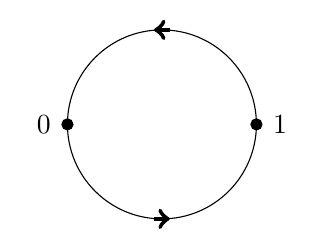
\begin{tikzpicture}
                \draw (0,0) circle(1.2cm);
                \draw[fill=black] (1.2,0) circle[radius=2pt];
                \draw[fill=black] (-1.2,0) circle[radius=2pt];
                \draw[->, ultra thick] (0.1,1.2)--(-0.1,1.2);
                \draw[->, ultra thick] (-0.1,-1.2)--(0.1,-1.2);
                \draw (1.5,0) node{1};
                \draw (-1.5,0) node{0};
            \end{tikzpicture}
        \end{center}

        Now start performing counterclockwise turns, and count how many times you go
        from 0 to 1, and from 1 to 0.

        If $C_{0\to 1}$ and $C_{1 \to 0}$ are the counts of going from 0 to 1 and from
        1 to 0 respectively, we have that if $C_{0\to 1}=C_{1\to 0}$, then $f(-1)=1$.
        Otherwise, we must have $f(-1)=0$.

        But having $C_{0\to 1}=C_{1\to 0}$ and that the total count is $C=C_{0\to
            1}+C_{1\to 0}$, means

        \[
            C=2C_{1\to 0}=2C_{0\to 1}
        \]

        Hence, $C$ is an even number. To verify that $S$ is dependent, we set $n=2r-1$
        for any integer $r$ and $t=-1$. With the results above, we can see that

        \[
            \sum_{k=0}^{2r-1}{c_k {(-1)}^{k}}=0
        \]

        if $c_1=c_2=\cdots=c_{2r-1}$, but not necessarily zero. This proves that $S$ is
        dependent.
    \end{proof}
\end{example}

\begin{theorem}
    Let $S=\{x_1,x_2,\dots,x_k\}$ an independent set formed by $k$ elements
    of a linear space $V$ and let $L(S)$ be the linear span of $S$. Then, any
    set of $k+1$ elements from $L(S)$ is dependent.
\end{theorem}

What this theorem says is that, taking any set of vectors in the linear span of
$S$, this is, formed by combining elements of $S$ (this vectors can be of any
nature), then, if we form a subset of the linear span of $S$ and it has more
elements than $S$ itself, the set will be dependent. This is because we are not
providing any new ``dimension'' to the new set. Say $S\in \mathbb{R^{3}}$, as
we are restricted to be in $\mathbb{R^{3}}$, taking $4$ vectors won't make any
object in $R^{i>3}$

\begin{proof}
    Let $T=\{y_1,y_2,\dots,y_{n+1}\}\subset L(S)$, this means that each $y_i$ is
    a linear combination of elements in $S$

    \[
        y_i=\sum_{j=1}^{n}{a_{ij}x_j}, \quad \textnormal{for } i=1,2,\dots,n+1
    \]

    For $T$ to be dependent, there must be some scalar set
    $C=\{c_1,c_2,\dots,c_{n+1}\}$, where not all of them are zero, that satisfies

    \[
        \sum_{i=1}^{n+1}{c_i y_i}=0
    \]

    We now want to prove by induction that for $n-1$ elements of $T$, there is a
    linear combination that satisfies dependency. Thus, we can try to form an
    equation that represents $T$ as a linear combination of $n-1$ elements. For
    this, we are going to take one element of $T$, multiply it by some scalar and
    subtract each element of $T$.

    Take the $1^{st}$ element in $T$ and multiply it by $c_i=\frac{a_{i1}}{a_{11}}$

    \[
        c_i y_1 = a_{i1}x_1 + \sum_{j=2}^{n}{c_i a_{1j} x_j}
    \]

    Now subtract $y_1$

    \begin{equation}
        \begin{split}
            c_i y_1 - y_i= a_{i1}x_1 + \sum_{j=2}^{n}{c_i a_{1j} x_j} - a_{i1}x1 +
            \sum_{j=2}^{n}{a_{ij}x_j}
            \\ = \sum_{j=2}^{n}{c_i a_{1j} x_j - a_{ij}x_j}
            \\ = \sum_{j=2}^{n}{\left(c_i a_{1j}- a_{ij}\right)x_j}
        \end{split}
    \end{equation}

    Equation (1.1) is indeed a linear combination of $n-1$ elements of $S$. By
    induction for $n$, we can prove that there are $n$ scalars
    $t_2,t_3,\dots,t_{n+1}$, that satisfy

    \begin{equation}
        \begin{split}
            \sum_{j=2}^{n+1}{t_i\left(c_i y_1- y_i\right)} = 0
        \end{split}
    \end{equation}

    As each $y_i$ is a linear combination of elements of $S$, we can write $y_i$ in
    terms of $y_1$.

    Equation (1.2) is solvable, because $y_i=c_i y_1$, this is true by the fact
    that $T\subset L(S)$.
\end{proof}

\section{Basis and dimension}
\begin{definition}
    A finite set $S$ of elements of a linear space $V$ is called a \textit{finite basis} of $V$ is $S$ is independent and spans $V$.
    $V$ is of finite dimension if it has a finite basis. Otherwise, $V$ has infinite dimension.
\end{definition}

\begin{theorem}
    Let $V$ be a linear space of finite dimension. Then any finite basis of $V$ has the same number of elements.
\end{theorem}

\begin{proof}
    This theorem can be proved with theorem $1.4$, let $S$ and $T$ be two finite bases for $V$, with $k$ and $m$ elements respectively.
    If $S$ generates $V$, then $V$ must have $k$ elements, we know that any set of $k+1$ elements of $V$ is dependent. Thus, $T$ must have
    $m\geq k$ elements. Applying the same reasoning vice-versa yields that $k=m$.
\end{proof}

This does not mean that a set of $k+1$ elements of $V$ can't span $V$. It
states that, the number of elements for a finite basis of a linear space $V$ of
dimension $k$, must have the same number of elements.

\begin{definition}
    If a linear space $V$ has a finite basis of $n$ elements, we write $n=\dim V$.
\end{definition}

The following theorem will not be proven. However, it has an intuitive
explanation.

\begin{theorem}
    Let $V$ be a linear space of finite dimension, with $\dim V = n$. Then

    \begin{enumerate}
        \item If $S$ is a finite basis for $V$, and $T$ is a set of independent elements of
              $V$, then $T\subseteq S$.
        \item Any set of $n$ independent elements of $V$ is a finite basis for $V$.
    \end{enumerate}

\end{theorem}

\section{Components}

Let $V$ be a linear space with $\dim V = n$, and consider an ordered basis

\[\left\{e_1, e_2,\dots,e_n\right\}\]
This ordered basis is considered as an n-tuple
$\left(e_1,e_2,\dots,e_n\right)$.

\begin{definition}
    An ordered basis of a linear space $V$ is a set of elements of $V$ that form a basis and provides information
    about the order of its elements.
\end{definition}

If $x\in V$, we can express $x$ as a linear combination of elements of the
basis

\begin{equation}
    \begin{split}
        x=\sum_{i=1}^{n}{c_i e_i}
    \end{split}
\end{equation}

This ensures that there is only one representation of $x$, take $x =
    \sum_{i=1}^{n}{c_i e_i}$, and $x = \sum_{i=1}^{n}{d_i e_i}$. Then

\[
    \sum_{i=1}^{n}{c_i e_i} = \sum_{i=1}^{n}{d_i e_i}
\]

Then $\sum_{i=1}^{n}{(c_i - d_i) e_i} = O$, where $O$ is the zero
vector/element of $V$. This means that $c_i=d_i$ for $i=1,2,\dots,n$. So there
is only one representation of $x$ in $V$.

\chapter{Euclidean spaces}

We start the section by defining what is a Euclidean space.

\begin{definition}
    A \textit{Euclidean space} is a finite-dimensional linear space that satisfies
    Euclidean geometry. They also are metric spaces, which are sets that have a notion
    of distance between its elements. Euclidean spaces are equipped with an \textit{inner product}.
\end{definition}

Euclidean spaces have a set of properties, that were defined as axioms in
\textit{Euclid's Elements}, which are
\begin{enumerate}
    \item If $a = b$ and $b = c$ then $a = c$ (the transitive property)
    \item If $a = b$ then $a + c = b + c$ (the equal sum property)
    \item If a line segment $\overline{AB}$ coincides in length and direction with
          $\overline{CD}$ then $\overline{AB} = \overline{CD}$.
    \item The whole is greater than the part. This can be thought as: \textit{let $A$ and
              $B\subset A$ be two arbitrary sets, then $A$ is ``bigger'' than $B$}.
    \item Things that are double of the same thing are equal to each other. (This one is
          very obvious, consider two equal circles with radius $r_1$ and $r_2$, then we
          can say that $r_1=r_2$).
\end{enumerate}

\section{Dot product and inner product}

\begin{definition}
    The \textit{inner product} is a function that maps two elements $x$ and $y$ from a linear space
    $V$ to a real number. We write the inner product as $\left(x,y\right)$.

    Any inner product satisfies the following properties:

    \begin{enumerate}
        \item $\left(x,y\right) = \overline{\left(y,x\right)}$ (hermitian symmetry)
        \item $\left(x,y+z\right) = \left(x,y\right) + \left(x,z\right)$ (linearity)
        \item $c\left(x,y\right) = \left(cx,y\right)$ (homogeneity)
        \item $\left(x,x\right) \geq 0$ (positive definite)
    \end{enumerate}

    \textbf{Remember}: a linear space with inner product is called a Euclidean space.
\end{definition}

\begin{example}[Inner product of two vectors in $\mathbb{R}^{2}$]

    \begin{center}
        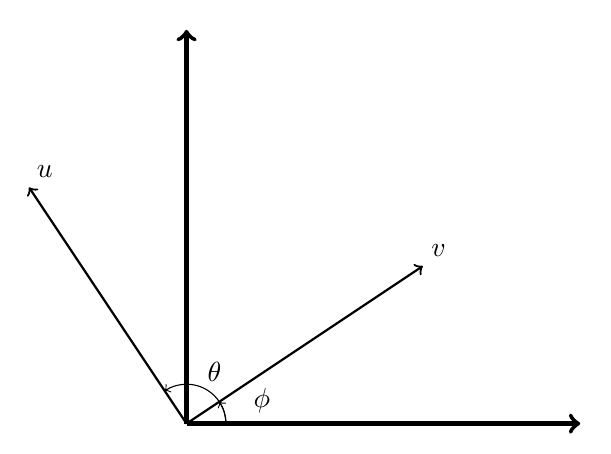
\begin{tikzpicture}
            \coordinate (u1) at (-2,3);
            \coordinate (u2) at (3,2);
            \coordinate (O) at (0,0);
            \coordinate (x) at (5,0);
            \coordinate (y) at (0,5);

            \draw[->, ultra thick] (O)--(x);
            \draw[->, ultra thick] (O)--(y);

            \draw[->, thick] (O)--(u1);
            \draw[->, thick] (O)--(u2);

            \draw (u1) + (.2,.2) node{$u$};
            \draw (u2) + (.2,.2) node{$v$};
            \pic [draw, ->, "$\theta$", angle eccentricity=1.5] {angle = x--O--u1};
            \pic [draw, ->, "$\phi$", angle eccentricity=2] {angle = x--O--u2};
        \end{tikzpicture}
    \end{center}

    Now, we have $u=\left(u_{x},u_{y}\right)$ and $v=\left(v_x, v_y\right)$. If we
    define the inner product of two vectors as

    \[
        \left(u,v\right) = u \cdot v = \sum_{i=1}^{n}{u_i v_i}
    \]

    For $n=2$, we have $u \cdot v = u_x v_x + u_y v_y$. We know the following
    relationships

    \begin{equation}
        \begin{split}
            \cos{\theta} = \frac{u_x}{|u|},\qquad
            \sin{\theta} = \frac{u_y}{|u|}
            \\\\
            \cos{\phi} = \frac{v_x}{|v|},\qquad
            \sin{\phi} = \frac{v_y}{|v|}
        \end{split}
    \end{equation}

    If we solve for $u$ and $v$ and substitute in the inner product formula, we get

    \begin{equation}
        \begin{split}
            u\cdot v = |u|\cdot|v|\cos\theta\cos\phi + |u|\cdot|v|\sin\theta\sin\phi
            \\ = |u||v|(\cos\theta\cos\phi + \sin\theta\sin\phi)
            \\ = |u||v|(\cos{\left(\theta - \phi\right)})
        \end{split}
    \end{equation}

    This means that the dot product of two vectors is the product of their length
    times the cosine of the angle between them. The angle between $u$ and $v$ is
    given by

    \begin{equation}
        \begin{split}
            \theta - \phi = \arccos{\left(\frac{u\cdot v}{|u| |v|}\right)}
        \end{split}
    \end{equation}

\end{example}

Well, this rises a question. How can you derive the inner product for a real
vector space? Well, there are various points to note, but let's imagine that we
want to measure the length of a vector. How can we measure distance? But also,
we want to measure the distance between two vectors. Let's go with an example
to make things clearer.

\begin{example}[Distance of two vectors in $\mathbb{R}^{n}$]
    We first define two vectors $u=\left(u_1,u_2,\dots,u_n\right)$ and $v=\left(v_1, v-2, \dots, v_n\right)$

    Now, a third vector, we call it $w=u-v$ has squared length
    \begin{equation}
        \begin{split}
            |w|^{2} = (u_1-v_1)^{2} + (u_2-v_2)^{2} + \cdots + (u_n-v_n)^{2}
        \end{split}
    \end{equation}

    Expanding one of the right-hand side terms we get $\left(u_i-v_i\right)^{2} =
        u_i^{2} - 2 v_i u_i + v_i^{2}$. Grouping the terms in (2.4) results in
    \begin{equation}
        \begin{split}
            \sum_{i=1}^{n}{\left(w_i^{2}\right)} = \sum_{i=1}^{n}{\left(u_i^{2}\right)} + \sum_{i=1}^{n}{\left(v_i^{2}\right)} - 2 \sum_{i=1}^{n}{u_i v_i}
        \end{split}
    \end{equation}

    Note that in (2.5) the dot product appears in the last term of the right-hand
    side. We can rewrite the equation as
    \begin{equation}
        \begin{split}
            w \cdot w = v \cdot v + u \cdot u - 2u \cdot v
        \end{split}
    \end{equation}

    And using formula (2.2)
    \begin{equation}
        \begin{split}
            |w|^{2} = |v|^{2} + |u|^{2} - 2|u||v|\cos\theta
        \end{split}
    \end{equation}

    Where $\theta$ is the angle between $u$ and $v$. Note that, because the angle
    between a vector and itself is $\theta = 0$, $\cos\theta = 1$.
\end{example}

Equation (2.7) is nothing more than the \textit{Law of Cosines}. Now, the dot
product does not follow a ``natural pattern'' as one would call it. Think of
the exponential function, it has a very natural reasoning, for example, in the
growth of populations or in differential equations. However, the dot product is
present when we measure elements in Euclidean spaces, like segments or vectors.

The dot product is not ``derived'' in a way most things are. Instead, it is
useful because it simply ``appears'' in measurements.

The \textbf{inner product} is a generalization of the dot product in more
general spaces. Each space can have a different definition for its inner
product. For example

    [Inner product of a functional space $C(a,b)$]

Let $f:\mathbb{R} \to \mathbb{R}$ and $g:\mathbb{R} \to \mathbb{R}$ be
continuous functions in an interval $[a,b]$, the inner product is defined as
\begin{equation}
    \begin{split}
        \left(f,g\right) = \int_{a}^{b}{f(x)g(x)dx}
    \end{split}
\end{equation}

\section{Norms and length}

The norm of an element $x$ in a linear space is written as $\|x\|$ and has the
following properties:

\begin{enumerate}
    \item $\|x\| > 0$ if $x\neq 0$
    \item $\|x\| = 0$ if $x = 0$
    \item For a scalar $a$, $\|ax\| = |a|\cdot \|x\|$
    \item For two elements $y$ and $x$ in a linear space, $\|x+y\| \leq \|x\| + \|y\|$
\end{enumerate}

The $4^{th}$ property is the triangle inequality.

\begin{definition}
    Let $x$ be an element of a linear space $V$.
    The norm of $x$ is defined as $\left(x,x\right)^{1/2}$, this is,
    the square root of the inner product of $x$ with itself.
\end{definition}

Definition (2.3) satisfies the properties of a norm.

\begin{example}
    Let $x\in\mathbb{R}^{n}$, the norm of a vector is given by the pythagorean theorem
    \begin{equation*}
        \begin{split}
            \|x\| = \sqrt{x_1^{2} + x_2^{2} + \cdots + x_n^{2}}
            = \sqrt{\sum_{i=1}^{n}{x_i^{2}}}
        \end{split}
    \end{equation*}

    Finally, we can see that $\|x\|=\sqrt{\left(x,x\right)}$, we defined the inner
    product of a real vector space as the dot product $\left(\cdot, \cdot\right):
        V\times V \to \mathbb{R}$. Here $V$ denotes the linear space, in our current
    example $V=\mathbb{R}^{n}$.
\end{example}

\begin{example}
    Let $V$ be the functional space $C(a,b)$, the norm of a function $f$ the interval $\left[a,b\right]$ is

    \begin{equation*}
        \begin{split}
            \|f\| = \sqrt{\int_{a}^{b}{\left[f(\psi)\right]^{2}d\psi}}
        \end{split}
    \end{equation*}

    This measure in functional spaces are useful when dealing with negative values
    on the integral. For example, the $\sin (\psi)$ function is zero when
    integrated in its period. However we can use the norm to measure it:

    \begin{equation*}
        \begin{split}
             & \|\sin(\psi)\| = \left(\sin(\psi), \sin(\psi)\right)
            \\                            & = \sqrt{\int_{\theta_1}^{\theta_2}{\left[\sin(\psi)\right]^{2}d\psi}}
            \\                            & = \sqrt{\left[\frac{\psi}{2} - \frac{\sin\left(2\psi\right)}{4}\right]_{\theta_1}^{\theta_2}}
            \\ &= \sqrt{\frac{\theta_1 + \theta_2}{2} - \frac{\sin(\theta_2)\cos(\theta_2)-\sin(\theta_1)\cos(\theta_1)}{2}}
        \end{split}
    \end{equation*}

    If $\theta_1=0$ and $\theta_2=2\pi$ we have $\|\sin(\psi)\|=\sqrt{\pi}$.
\end{example}

\begin{theorem}
    In the Euclidean space $V$, every inner product satisfies the Cauchy-Schwarz inequality:

    \begin{equation}
        |\left(x,y\right)|^{2} \leq \left(x,x\right)\left(y,y\right)
    \end{equation}
\end{theorem}

\begin{proof}
    Let $z=ax+by$. If $x=0$ and $y=0$ the problem is trivial and the equality holds. Else, we can use
    the fact that $\left(z,z\right) \geq 0$ and by using the properties of the inner product:
    \begin{equation*}
        \begin{split}
             & \left(z,z\right) = \left(ax+by, ax+by\right)
            \\        & = \left(ax,ax\right) + \left(ax,by\right) + \left(by,ax\right) +\left(by,by\right)
            \\        & = a\bar{a}\left(x,x\right) + a\bar{b}\left(x,y\right) + b\bar{a}\left(y,x\right) + b\bar{b}\left(y,y\right)
            \\  &\geq 0
        \end{split}
    \end{equation*}

    Now, let $a = \bar{a} = (y,y)$
    \begin{equation*}
        \begin{split}
            \left(y,y\right)\left(y,y\right)\left(x,x\right) + \bar{b}\left(y,y\right)\left(x,y\right) + b\left(y,y\right)\left(y,x\right) + b\bar{b}\left(y,y\right)
            \geq 0
        \end{split}
    \end{equation*}

    Dividing everything by $\left(y,y\right)$ leaves
    \begin{equation*}
        \begin{split}
            \left(y,y\right)\left(x,x\right) + \bar{b}\left(x,y\right) + b\left(y,x\right) + b\bar{b}
            \geq 0
        \end{split}
    \end{equation*}

    If we let $b = -\left(x,y\right)$, such that its conjugate $\bar{b} =
        -\left(y,x\right)$, we obtain
    \begin{equation*}
        \begin{split}
             & \left(x,x\right)\left(y,y\right) - \left(x,y\right)\left(y,x\right) - \left(x,y\right)\left(y,x\right) + \left(x,y\right)\left(y,x\right)
            \\  &\left(x,x\right)\left(y,y\right) - \left(x,y\right)\left(y,x\right) \geq 0
        \end{split}
    \end{equation*}

    If we reorder the terms of this equation, we are left with the Cauchy-Schwarz
    inequality
    \begin{equation*}
        \left(x,y\right)\left(x,y\right) \leq \left(x,x\right)\left(y,y\right)
    \end{equation*}
\end{proof}

\begin{example}
    Applying theorem (2.1) in $C(a,b)$, with inner product $\left(f,g\right)=\int_{a}^{b}{f(t)g(t)dt}$, results in

    \begin{equation*}
        {\left(\int_{a}^{b}{f(t)g(t)dt}\right)}^{2} \leq \left(\int_{a}^{b}{{\left[f(t)\right]}^{2}dt}\right)\left(\int_{a}^{b}{{\left[g(t)\right]}^{2}dt}\right)
    \end{equation*}
\end{example}

The triangle inequality is a direct consequence of the Cauchy-Schwarz
inequality, see
\begin{proof}[The triangle inequality]
    Let $x,v\in V$ where $V$ is an Euclidean space. With the properties of the inner product we can see that
    \begin{equation}
        \begin{split}
             & \|x+y\|^{2} = \left(x+y,x+y\right)
            \\        & = \left(x,x\right) + \left(x,y\right) + \left(y,x\right) + \left(y,y\right)
            \\  & = \left(x,x\right) + \left(x,y\right) + \overline{\left(x,y\right)} + \left(y,y\right)
        \end{split}
    \end{equation}
\end{proof}

The sum $\left(x,y\right) + \overline{\left(x,y\right)}$ is real, see
\begin{equation*}
    z = a + bi \longrightarrow \bar{z} = a - bi, \textnormal{ such that } z + \bar{z} = 2a
\end{equation*}

So, we can use the Cauchy-Schwarz inequality. See that $\|(x,y)\|^{2}\leq
    \|x\|\|y\|$ and $\|(y,x)\|^{2} = \|\overline{(x,y)}\|^{2} \leq \|x\|\|y\|$.
Transforming (2.10) into an inequality holds
\begin{equation*}
    \begin{split}
        \|x+y\|^{2}=\left(x,x\right) + \left(x,y\right) + \overline{\left(x,y\right)} + \left(y,y\right)
        \\  = \|x\|^{2} + \|y\|^{2} + \left(x,y\right) + \overline{\left(x,y\right)}
        \\  \leq  \|x\|^{2} + \|y\|^{2} + 2\|x\|\|y\|
    \end{split}
\end{equation*}

You can easily see that $\|x\|^{2} + \|y\|^{2} + 2\|x\|\|y\| =
    (\|x\|+\|y\|)^{2}$. We get
\begin{equation}
    \|x+y\|^{2} \leq (\|x\|+\|y\|)^{2}
\end{equation}

This proves the triangular inequality
\begin{equation*}
    \|x+y\| \leq \|x\|+\|y\|
\end{equation*}

\begin{definition}
    In a real Euclidean space $V$, the angle between two non-null elements $x$ and $y$ is defined as the number $\theta$
    in the interval $\left[0,\pi\right]$. This number satisfies the following equation
    \begin{equation}
        \cos\theta = \dfrac{\left(x,y\right)}{\|x\|\|y\|}
    \end{equation}
\end{definition}

By using the Cauchy-Schwarz inequality in (2.4) we can prove that
\begin{equation*}
    \begin{split}
        \|(x,y)\|^{2} = \|x\|^{2}\|y\|^{2}\cos^{2}\theta \leq \|x\|\|y\|
    \end{split}
\end{equation*}

Such that $\|x\|\|y\|\cos^{2}\theta \leq 1$. But we know that $\|x\|\geq 0$ and
$\|y\|\geq 0$, so
\begin{equation*}
    0 \leq \|x\|\|y\|\cos^{2}\theta \leq 1
\end{equation*}

This is the same as
\begin{equation*}
    0 \leq \|(x,y)\|^{2} \leq 1
\end{equation*}

Thus, $-1 \leq (x,y) \leq 1$. This proves that the quotient in the right-hand
side of (2.12) is in $[-1,1]$, so $\cos\theta$ will go from $[0,\pi]$.

\chapter{Projections onto subspaces}

A projection is an idempotent mapping of a set (or any structure) into a subset
(or sub-structure). Idempotent means that, projecting once is the same as
projecting $n$-times.

We will see this as a vector being projected in a line, a line is a subspace of
$\mathbb{R}$, and our vector is in $\mathbb{R}^{2}$.

\begin{center}
    \begin{tikzpicture}
        \coordinate (v) at (2,3);
        \coordinate (e) at (14/5, 7/5);
        \coordinate (l1) at (-2,-1);
        \coordinate (l2) at (4,2);

        \draw[thick, dashed] (l1)--(l2);
        \draw[->, thick] (0,0)--(0,5);
        \draw[->, thick] (0,0)--(5,0);
        \draw[->, very thick] (0,0)--(v);
        \draw[dashed] (v)--(e);
        \draw[->, very thick] (0,0)--(e);

        \draw (l2) + (0.2,0.2) node{$l$};
        \draw (e) + (0, 1) node{$e$};
        \draw (v) + (-1, -1) node{$v$};
        \draw (e) + (-.9, -.9) node{$proj_u {v}$};

    \end{tikzpicture}
\end{center}

This is the most basic example of projection. Let's deduce a formula.

\begin{example}
    Let $v\in\mathbb{R}^{2}$ and let $l$ be a line
    in $\mathbb{R}^{2}$ parametrized by a vector $u$ as $f(t)=ut$.

    \begin{center}
        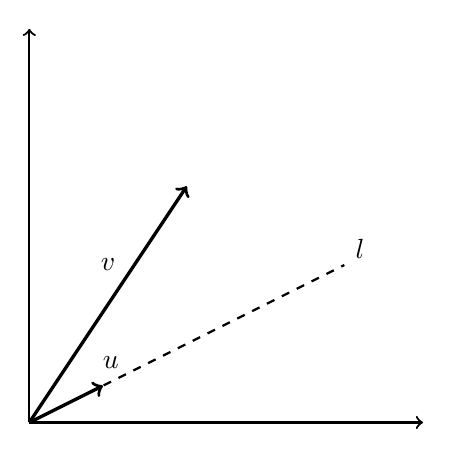
\begin{tikzpicture}
            \coordinate (v) at (2,3);
            \coordinate (e) at (14/15, 7/15);
            \coordinate (l1) at (0,0);
            \coordinate (l2) at (4,2);

            \draw[thick, dashed] (l1)--(l2);
            \draw[->, thick] (0,0)--(0,5);
            \draw[->, thick] (0,0)--(5,0);
            \draw[->, very thick] (0,0)--(v);
            \draw[->, very thick] (0,0)--(e);

            \draw (l2) + (0.2,0.2) node{$l$};
            \draw (v) + (-1, -1) node{$v$};
            \draw (e) + (.1,.3) node{$u$};

        \end{tikzpicture}
    \end{center}

    What we want to find is some constant $k$ such that $ku$ is perpendicular to
    $l$. We know from the previous image that $e=proj_u v - v = uk-v$

    \begin{equation*}
        \begin{split}
            (ku-v)\cdot u = k\|u\|^{2} - v\cdot u = 0
        \end{split}
    \end{equation*}

    Then $k=\frac{v\cdot u}{\|u\|^{2}}$. The formula for projection becomes

    \begin{equation}
        \begin{split}
            proj_u v = ku = \frac{v\cdot u}{\|u\|^{2}}\cdot u
        \end{split}
    \end{equation}

    We call this projection in terms of $u$, because $l$ is parametrized by $u$.
\end{example}

Now, we want to extend this idea to any linear space. We can see that a
projection is a multiplication of the ``projection basis'' by some scalar.

This gives us an idea of what the inner product is: we can think of the inner
product as ``how much of some element is onto other element''. Think of
projecting a vector $v$ onto $u$ when $v\perp u$.

\begin{center}
    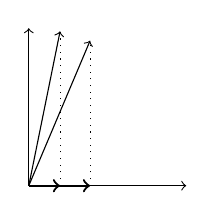
\begin{tikzpicture}
        \coordinate (v) at (2,0);
        \coordinate (e) at (0,2);
        \coordinate (c) at (0.778836684617, 1.84212198801);
        \coordinate (d) at (0.39733866159, 1.96013315568);

        \draw[->] (0,0)--(v);
        \draw[->] (0,0)--(e);
        \draw[->] (0,0)--(c);
        \draw[->] (0,0)--(d);
        \draw[dotted] (0.39733866159,0) -- (d);
        \draw[dotted] (0.778836684617,0) -- (c);
        \draw[->, thick] (0,0) -- (0.778836684617,0);
        \draw[->, thick] (0,0) -- (0.39733866159,0);
    \end{tikzpicture}
\end{center}

You can see that the projection tends to a vector with no length. This can be
proven easily with (2.2):

\begin{equation}
    \begin{split}
        proj_u v = u\cdot\frac{u\cdot v}{\|u\|^{2}}
        \\ = u\cdot\frac{\|v\|}{\|u\|} \cos\psi
    \end{split}
\end{equation}

The $\frac{\|v\|}{\|u\|}$ part is the amount of times $u$ fits in $v$, and if
$\psi = \frac{\pi}{2}$ then the projection is the $O$ vector.

\begin{example}[Projections in $\mathbb{R}^{n}$]
    Let $x\in\mathbb{R}^{n}$ be a vector in a plane, this plane must be of dimension $n-1$.
    Thus, it has a basis with $n-1$ elements given by
    \begin{equation*}
        W = \left(e_1, e_2,\dots, e_{n-1}\right)
    \end{equation*}

    Where $e_1,e_2,\dots,e_{n-1}\in\mathbb{R}^{n}$. These vectors parametrize the
    plane, such that $x$ can be written as
    \begin{equation}
        \begin{split}
            x = \sum_{i=1}^{n-1}{c_i e_i}
        \end{split}
    \end{equation}

    for any scalars $c_1,c_2,\dots,c_{n-1}$. Now, suppose that we have a vector
    $v\in\mathbb{R}^{n}$ that preferably, does not lie in this plane.

    To find the projection, we can set a set of equation that are analogous to the
    example in $\mathbb{R}^{2}$:
    \begin{equation}
        \begin{split}
            \begin{cases}
                e_1(v - k x) = 0 \\
                e_2(v - k x) = 0 \\
                \cdots           \\
                e_{n-1}(v - k x) = 0
            \end{cases}
        \end{split}
    \end{equation}

    Where $k\in\mathbb{R}$. What we want is to make each basis vector orthogonal to
    a vector $x$ that connects $v$ to the plane. In other words, the vector
    $(v-kx)$ will be perpendicular to the plane.

    We will collect each basis vector into a matrix
    \begin{equation}
        A = \left[
            \begin{matrix}
                \vdots & \vdots &        & \vdots  \\
                e_1    & e_2    & \cdots & e_{n-1} \\
                \vdots & \vdots &        & \vdots  \\
            \end{matrix}
            \right]
    \end{equation}

    Here, $A$ has dimension $n\times (n-1)$. The system of equations in (3.4)
    becomes
    \begin{equation}
        A^{T}\left(v-kx\right) = 0
    \end{equation}

    But we can rewrite $x$ as a vector $c$ times $A$, so that
    \begin{equation}
        x = Ac =  \left[\begin{matrix}
                \vdots & \vdots &        & \vdots  \\
                e_1    & e_2    & \cdots & e_{n-1} \\
                \vdots & \vdots &        & \vdots  \\
            \end{matrix}\right]\cdot\left[\begin{matrix}
                c_1 \\c_2\\\vdots\\c_{n-1}
            \end{matrix}\right]
    \end{equation}

    You can verify that this is the same as writing $x$ in the form (3.3).
    Rewriting equation (3.6) leaves
    \begin{equation*}
        A^{T}\left(v-Ac\right) = 0
    \end{equation*}

    We omit the term $k$ since we will assume that the vector $c$ scales $x$
    accordingly. Expanding the equation
    \begin{equation}
        \begin{split}
            A^{T}\left(v-Ac\right) = A^{T}v - A^{T}Ac = 0
        \end{split}
    \end{equation}

    Now, we solve for $c$
    \begin{equation}
        \begin{split}
            c={(A^{T}A)}^{-1}A^{T}v
        \end{split}
    \end{equation}

    Now, as the projection is given by scaling all the basis vectors in $A$ by $c$
    (think of $c$ as the scalar term in the 2-dimensional example), we can write
    our projection vector $p$ as

    \begin{equation}
        p = Ac = A{(A^{T}A)}^{-1}A^{T}v = Pv
    \end{equation}

    We define $P$ to be the \textbf{projection matrix}, and $v$ is the vector
    projected onto the plane $A$.

    To figure out the equation of the plane, we think of the definition of a plane:
    each vector in the plane must be perpendicular to a normal vector. This means
    that we always have $A\cdot n = O$, where $n$ is the normal vector.

    We can write the equation for an hyperplane in $\mathbb{R}^{n-1}$ as
    \begin{equation}
        n^{T}(x-x_0) = 0
    \end{equation}

    where:
    \begin{itemize}
        \item $n \in \mathbb{R}^n$ is the \textbf{normal vector} to the hyperplane,
        \item $x \in \mathbb{R}^n$ is any point \textbf{on} the hyperplane,
        \item $x_0 \in \mathbb{R}^n$ is a fixed point in the hyperplane (used to position or ``anchor'' the hyperplane in space).
    \end{itemize}

    This equation states that the vector from $x_0$ to any point $x$ on the
    hyperplane is \textbf{orthogonal} to the normal vector $n$, ensuring all such
    points lie in the same flat $(n-1)$-dimensional space.

    In this definition we didn't use the basis vectors in $W$, however as $x$ is a
    combination of basis vectors, it is not necessary to explicitly write them.
\end{example}

Some important applications of projections are \textbf{linear regression}, or
the \textbf{Fourier series} we will see how to derive them later.

% TODO: Fourier series %

\begin{example}[Linear Regression]
    Let $S$ be a set of points in $\mathbb{R}^{n-1}$, suppose we can map the points
    with a scalar field given by $f:\mathbb{R}^{n-1}\to\mathbb{R}$, this means that
    $S$ can be written as:
    \begin{equation}
        \begin{split}
            S = \left\{\left(x_{11},x_{12},\dots,x_{1(n-1)},z_{1} \right), \dots, \left(x_{m1}, x_{m2},\dots,x_{m(n-1)}, z_m\right)\right\}
        \end{split}
    \end{equation}

    We can set a system of equations that uses a coefficient vector $u$ and a
    \textit{bias}:
    \begin{equation}
        \begin{cases}
             & x_{11}u_1 + x_{12}u_2 + \cdots + x_{1(n-1)}u_{n-1} + b = z_1
            \\                                                                                                                                                           & x_{21}u_1 + x_{22}u_2 + \cdots + x_{2(n-1)}u_{n-1} + b = z_2
            \\                                                                                                                                                           & \qquad \qquad \qquad \qquad \vdots
            \\ &x_{m1}u_1 + x_{m2}u_2 + \cdots + x_{m(n-1)}u_{n-1} + b = z_m
        \end{cases}
    \end{equation}

    Each $z$ is a combination of $n-1$ independent variables, plus a bias term. We
    can rewrite the system as an $m\times n$ matrix multiplied by an $n\times 1$
    vector
    \begin{equation}
        \left[
            \begin{matrix}
                1      & x_{11} & x_{12} & \cdots & x_{1(n-1)} \\
                1      & x_{21} & x_{22} & \cdots & x_{2(n-1)} \\
                \vdots & \vdots & \vdots & \ddots & \vdots     \\
                1      & x_{m1} & x_{m2} & \cdots & x_{m(n-1)} \\
            \end{matrix}
            \right]\cdot \left[
            \begin{matrix}
                b \\ u_1 \\\vdots\\u_{n-1}
            \end{matrix}
            \right] = \left[
            \begin{matrix}
                z_1 \\z_2\\\vdots\\z_m
            \end{matrix}
            \right]
    \end{equation}
    \begin{equation*}
        X\cdot u = z
    \end{equation*}

    We want to fit the equation to an approximation vector $\hat u$. The vector $z$
    lies in a hyperplane. $\hat u$ is essentially a vector that gives the direction
    of a line that fits these points at best. This works because, the projection
    gives the minimum distance to $z$.
    \begin{equation}
        \hat u = {\left(X^{T}X\right)}^{-1}X^{T}z
    \end{equation}

    But this approximation only has one dimension for the output. If you let $z$ be
    a matrix, so that each output of the system of equations is a vector, then
    define $u$ to be a $n\times p$ matrix and $z$ to be $m\times p$.
    \begin{equation}
        \left[
            \begin{matrix}
                1      & x_{11} & \cdots & x_{1(n-1)} \\
                1      & x_{21} & \cdots & x_{2(n-1)} \\
                \vdots & \vdots & \ddots & \vdots     \\
                1      & x_{m1} & \cdots & x_{m(n-1)} \\
            \end{matrix}
            \right]\cdot \left[
            \begin{matrix}
                b_1        & \cdots & b_p        \\
                u_{11}     & \cdots & u_{1p}     \\
                \vdots     & \ddots & \vdots     \\
                u_{(n-1)1} & \cdots & u_{(n-1)p} \\
            \end{matrix}
            \right] = \left[
            \begin{matrix}
                z_{11} & \cdots & z_{1p} \\
                z_{21} & \cdots & z_{2p} \\
                \vdots & \ddots & \vdots \\
                z_{m1} & \cdots & z_{mp} \\
            \end{matrix}
            \right]
    \end{equation}

    Then $\hat u$ has dimension $n \times p$, defining a hyperplane that best fits
    the data in $X$ across all output dimensions.

    While $\hat u$ provides an approximation for each point in $X$, the hyperplane
    must fit all points. In an $n$-dimensional space, this requires only $n$
    coefficients.

    For that, we can take the mean of each row (as we have $n$ rows) and
    approximate a plane with the following equation:
    \begin{equation}
        \begin{split}
            P(x_1, x_2, \dots, x_{n-1}) = \bar{b} + \bar{u}_1 x_1 + \cdots + \bar{u}_{n-1} x_{n-1}        \end{split}
    \end{equation} Where
    \begin{itemize}
        \item $\bar{b} = \dfrac{1}{p}\sum_{i=1}^{p}{b_i}$
        \item $\bar{u}_i = \dfrac{1}{p}\sum_{j=1}^{p}{u_{i j}}$ for $\,i\in\left\{1,2,\dots,n-1\right\}$
    \end{itemize}

    \textbf{Worked example: } Suppose that we have a set of points given in the table below:

    \begin{center}
        \begin{tabular}{|c|c|c|c|c|}
            \hline
            \textbf{Point} & $x_1$ & $x_2$ & $z^{(1)}$ & $z^{(2)}$ \\
            \hline
            1              & 2     & 3     & 10        & 11        \\
            2              & 6     & 7     & 9         & 8         \\
            3              & 4     & 2     & 7         & 9         \\
            \hline
        \end{tabular}
    \end{center}

    Note that we have two different outputs, namely $z^{(1)}$ and $z^{(2)}$. This
    is because we can have multiple readings for the same inputs $x_1,x_2$.

    Now, using the method described above we can set up our system of equations
    \begin{equation}
        \begin{split}
            X\cdot u = z \\[1em]
            \begin{bmatrix}
                1 & 2 & 3 \\
                1 & 6 & 7 \\
                1 & 4 & 2 \\
            \end{bmatrix}
            \cdot
            \begin{bmatrix}
                b_1    & b_2    \\
                u_{11} & u_{12} \\
                u_{21} & u_{22}
            \end{bmatrix}
             & =
            \begin{bmatrix}
                10 & 11 \\
                9  & 8  \\
                7  & 9  \\
            \end{bmatrix}
        \end{split}
    \end{equation}

    Solving for $\hat{u} = \left(X^{T}X\right)^{-1}X^{T}z$:
    \[
        \hat{u} =
        \begin{bmatrix}
            9.6667  & 12.3333 \\
            -1.0833 & -0.9167 \\
            0.8333  & 0.1667
        \end{bmatrix}
    \]

    Now, we take the mean of each row and convert it to a column vector $\bar{u}$
    \[
        \bar{u} = \left[
            \begin{matrix}
                \bar{b} \\\bar{u}_1\\\bar{u}_2
            \end{matrix}
            \right] = \left[
            \begin{matrix}
                11 \\ -1 \\ 0.5
            \end{matrix}
            \right]
    \]

    This gives a final approximation
    \[
        P(x, y) = 11 - x + \dfrac{1}{2}y
    \]
\end{example}

\section{Orthogonalization}

Formally, orthogonalization is the process of taking a set of independent
vectors in some linear space $V$ and transforming them into an orthogonal
basis. We define an orthogonal basis as

\begin{definition}
    An orthogonal basis of a linear space $V$ is a set of $n=\dim V$ elements, called
    $S=\left\{v_1,v_2,\dots,v_n\right\}$ such that the inner product

    \begin{equation}
        \left(v_i, v_j\right) = 0, \textnormal{ if } i\neq j
    \end{equation}
\end{definition}

\begin{example}
    We commonly define the basis of vector spaces like $\mathbb{R}^{2}$, $\mathbb{R}^{3}$, \dots, $\mathbb{R}^{n}$ to be orthogonal.
    We denote their elements as $e_1, e_2,\dots, e_n$.
\end{example}

The \textbf{Gram-Schmidt} process converts a set of $n$ independent elements to
an orthogonal basis for the space that they span.

\section{Gram-Schmidt orthogonalization}

Let $X=\left\{x_1, x_2,\dots,x_n\right\}$ be a set of independent elements of a
linear space $V$. We want to build an orthogonal basis
$Y=\left\{y_1,y_2,\dots,y_n\right\}$ in $V$.

To do so, we start by taking the first element of $X$. Let $y_1 = x_1$ be the
first element of the basis. The rest of the elements will be built around this
one.

If we take the second element, namely $x_2$, and we project $x_2$ onto $y_1$,
you can easily check (by drawing it) that the vector $x_2 -
    \textnormal{proj}_{y_1}{x_2}$ is orthogonal to $x_1$. You can see the
projection formula derivation in the previous section. With this, we define
$y_2 = x_2 - \frac{\left(x_2,y_1\right)}{\left(y_1,y_1\right)}y_1$.

Now, we have a basis of two vectors. Geometrically, it represents a plane. The
third vector will not be coplanar to these two, because of their independency.
Thus, we can project the vector onto the plane by combining both projections
onto $y_1$ and $y_2$. So $y_3 = x_3 - \left(\textnormal{proj}_{y_2}{x_3}+
    \textnormal{proj}_{y_1}{x_3}\right)$.

In figure $3.1$ you can see a graphical description. The orthogonal basis is
$b_1,b_2,b_3$. Take a closer look at $a_3$, this is the third independent
vector, $c_3$ is a linear combination of $c_{32}$ and $c_{31}$, who are the
projections of $a_3$ onto $b_1$ and $b_2$. You can think of these projections
as the ``components'' of $a_3$ in the direction of $b_1$ and $b_2$. Thus, the
sum of those components form $c_3$, and $a_3 - c_3$ is a vector orthogonal to
$b_1$ and $b_2$.

\begin{figure}
    \caption{Gram-Schmidt orthogonalization in $\mathbb{R}^{3}$}
    \centering
    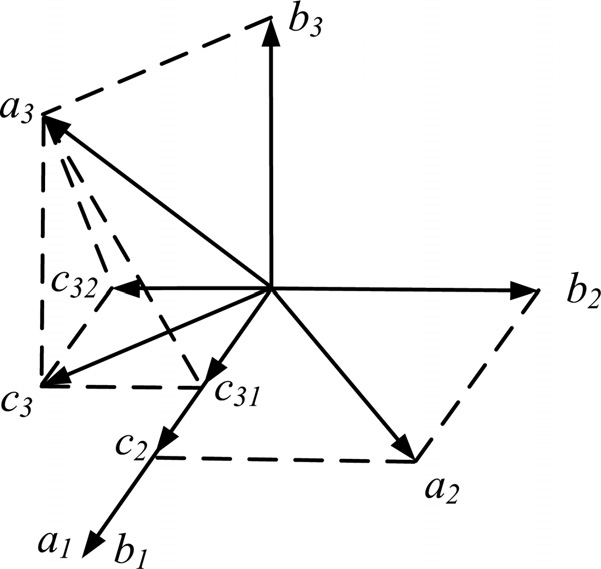
\includegraphics[width=0.25\textwidth]{An-illustration-of-Gram-Schmidt-transformation}
\end{figure}

To find all the vectors, we can write the following equations. For $r = 1, 2,
    \dots, n-1$ we have
\begin{equation}
    y_1 = x_1
\end{equation}
\begin{equation}
    y_{r+1} = x_{r+1} - \sum_{i=1}^{r}{\dfrac{\left(x_{r+1}, y_i\right)}{\left(y_i, y_i\right)}x_{r+1}}
\end{equation}

Or, alternatively
\begin{equation}
    y_{r+1} = x_{r+1} - \sum_{i=1}^{r}{\textnormal{proj}_{y_i}{x_{r+1}}}
\end{equation}

These are the formulas for \textbf{Gram-Schmidt} orthogonalization.

\begin{example}[Fourier Series]
    To approximate continuous functions in an interval $\left[0,2\pi\right]$, Fourier discovered that
    he could combine trigonometric polynomials. Let $V=C(0,2\pi)$ the linear space of all real continuous functions
    in the interval $\left[0,2\pi\right]$, we define the inner product as $\left(f,g\right) = \int_{a}^{b}{f(x)g(x)dx}$.

    Now, we try to find a normal set of trigonometric functions, this are the basis
    elements of our linear space. First, consider the functions $\cos{kx}$ and
    $\sin{kx}$. In a previous section we've seen that the norm of these functions
    is $\sqrt \pi$. Now, define a finite set of $n$ elements consisting of these
    trigonometric functions, and define them as $\psi_0, \psi_1, \dots$ where
    \begin{equation}
        \psi_0(x) = \dfrac{1}{\sqrt{2\pi}}, \quad \psi_{2k-1}(x) = \dfrac{\cos{kx}}{\sqrt{\pi}}, \quad \psi_{2k}(x) = \dfrac{\sin{kx}}{\sqrt{\pi}}
    \end{equation}

    for $k \geq 1$. You can check that $\left(\psi_{2k-1},
        \psi_{2k}\right)=\dfrac{1}{\pi}\int_{0}^{2\pi}{\cos{(kx)}\sin{(kx)}dx} = 0$ for
    all $k$. Also, for two elements $p,q\leq \dim V$ where $p\neq q$, we have that
    \begin{equation}
        \begin{split}
            \dfrac{1}{\pi}\int_{0}^{2\pi}{\cos(px)\cos(qx)dx} = 0 \\[1em]
            \dfrac{1}{\pi}\int_{0}^{2\pi}{\sin(px)\sin(qx)dx} = 0
        \end{split}
    \end{equation}

    Thus, the set $\Psi =
        \left\{\psi_0,\psi_1,\dots,\psi_{2k-1},\psi_{2k},\dots\right\}$ is a normalized
    orthogonal basis of $V$.

    These elements span a subspace $S$, so $S = L\left(\psi_0,\psi_1,\dots\right)$.
    If we want to approximate a function $f$, we must take the projection of $f$
    onto $S$. Let $f_n$ be the projection onto an $n$ dimensional subspace $S$
    spanned by the elements of $\Psi$:
    \begin{equation}
        f_n = \sum_{k=1}^{n}{(f, \psi_k)\psi_k}, \quad\textnormal{where }(f,\psi_k) = \int_{0}^{2\pi}{f(x)\psi_k(x)\,dx}
    \end{equation}
    Note that we omit the coefficient $\frac{1}{(\psi_k,\psi_k)}$, as $\psi_k$ is normalized it has norm $1$.

    Using the formulas in (3.23) we can write (3.25) as
    \begin{equation}
        f_n(x) = a_0 + \sum_{k=1}^{n}\left({a_k \cos{kx} + b_k \sin {kx}}\right)
    \end{equation}
    where
    \begin{equation}
        \begin{split}
             & a_0 = \dfrac{1}{2\pi}\int_{0}^{2\pi}{f(x)\,dx}        \\[1em]
             & a_k = \dfrac{1}{\pi}\int_{0}^{2\pi}{f(x)\cos(kx)\,dx} \\[1em]
             & b_k = \dfrac{1}{\pi}\int_{0}^{2\pi}{f(x)\sin(kx)\,dx}
        \end{split}
    \end{equation}

    \textbf{Fourier series} can be written as
    \begin{equation}
        f(x) = a_0 + \sum_{k=1}^{\infty}\left({a_k \cos{kx} + b_k \sin {kx}}\right)
    \end{equation}
\end{example}

\chapter{Linear Transformations}

\section{Definition}
A transformation is a function whose domain and image are subspaces of a linear
space. Let $T$ be a transformation, we denote
\begin{equation}
    T: V \to W
\end{equation}
to say that $T$ maps
elements from its domain, $V$, to its image, $W$. Remember, $V$ is any linear space and $W$ is a
subset of that linear space.

A linear transformation is a kind of transformation that follows certain
properties. Let $T: V\to W$ be a linear transformation, then
\begin{enumerate}
    \item T(x+y) = T(x)+T(y)
    \item T(cx) = cT(x)
\end{enumerate}
for $x,y\in V$ and $c\in \mathbb{R}$.

Both properties can be combined to get
\begin{equation*}
    T(ax+by) = aT(x)+bT(y),
\end{equation*}
which can be generalized as
\begin{equation}
    T\left(\sum_{i=1}^{n}{k_i x_i}\right) = \sum_{i=1}^{n}{k_i T(x_i)}
\end{equation}
for $x_1,x_2,\dots, x_n\in V$ and $k_1,k_2,\dots,k_n \in \mathbb{R}$.

\section{Kernel and range}

We must recap some concepts from the previous chapters. We know that any linear
space must have a \textit{zero element}, commonly we will denote this element
as $O$.

Linear transformations map from a subspace to another subspace of the same
linear space. The definition of a subspace given in theorem 1.4.1 says that any
subspace $S$ of a linear space $V$ must satisfy the ten axioms of closure.
Axiom 5 says that there must be a zero element, so any transformation must map
the zero element.

There will be a subset in the domain of $T$ that will map this element. This is
called \textbf{kernel}.

\begin{definition}
    The \textbf{kernel} of a linear transformation $T: V\to W$ is a subset $K\subseteq V$ such that
    \begin{equation}
        K(T) = \left\{x: x\in V \wedge T(x)=0\right\}
    \end{equation}
\end{definition}

As any subspace, $T(V)$ spans another subspace. This is called the
\textbf{range} of $T$.

\begin{theorem}
    The set $T(V)$ (range of $T$) is a subspace of $W$.
    Furthermore, $T$ maps the zero element on $V$ to the zero element of $W$.
\end{theorem}

\begin{proof}
    Let $e_1,e_2,\dots,e_n\in V$ be independent, and $k_1,k_2,\dots,k_n\in \mathbb{R}$.
    We can form every element in $V$ as a combination of these elements. Let $y$ be any
    element in $V$ given by
    \begin{equation*}
        y = \sum_{i=1}^{n}{k_i e_i},
    \end{equation*}
    then we have $T(y)\in W$. If this applies for any $y$, then it does for any element in $V$.

    Now, to prove the second sentence, let $x\in V$ and $c\in \mathbb{R}$. The
    transformation $T(cx)=0$, then $cT(x) = 0$ if $c=0$ for any $x$ ($0x=O$).
\end{proof}

\subsection{Dimension of the kernel and range of a transformation}

We are interested in the relationship between the dimension of $K(T)$ and
$T(V)$. For this, we present the following theorem.

\begin{theorem}[Rank-Nullity Theorem]
    If $V$ is a linear space of finite dimension. Let $T$ be a linear transformation, then $T(V)$ must be finite and we have
    \begin{equation}
        \dim N(T) + \dim K(T) = \dim V
    \end{equation}
\end{theorem}

\begin{proof}
    Let $n=\dim V$, and $e_1,e_2,\dots,e_k$ be a basis for $K(T)$, where
    $k=\dim K(T)$. A basis of $V$ can be
    \begin{equation*}
        e_1,\dots,e_k,e_{k+1},\dots,e_{k+r}
    \end{equation*}
    where $k+r=n$.

    If we take an element $y$ from $V$, we can write it as
    \begin{equation*}
        y=\sum^{k+r}_{i=1}{c_i e_i}, \quad \textnormal{for any scalars } c_1,c_2,\dots,c_{k+r}
    \end{equation*}

    If we apply the transformation, we get
    \begin{equation*}
        T(y)=T\left(\sum^{k+r}_{i=1}{c_i e_i}\right) = \sum^{k+r}_{i=k+1}{c_i T(e_i)}
    \end{equation*}
    Note that we have changed $i$ to be $k+1$, because $T(e_1) = \cdots = T(e_k) = O$.

    This proves that any element in $T(V)$ is a combination of $r$ independent
    elements, so $r=\dim T(V)$, which proves the theorem.
\end{proof}

Now, we are going to give an example with infinite linear spaces.

\begin{theorem}
    Let $V$ be a linear space of \textbf{infinite dimension}.
    Let $T$ be a linear transformation $T: V\to W$. Then at least
    $T(V)$ (image of $T$) or $K(T)$ (kernel of $T$) must have infinite
    dimension.
\end{theorem}

\begin{proof}
    Suppose that
    \begin{equation*}
        \begin{cases}
            \dim T(V) = r \\
            \dim K(T) = k
        \end{cases}
    \end{equation*}

    Now, let $e_1,\dots,e_k$ be a base for $K(T)$. And let a base for $V$ be
    \begin{equation*}
        e_1,\dots,e_k,e_{k+1},\dots,e_{k+n},
    \end{equation*}
    where $n > r$. By contradiction, we want to prove that this is not
    possible. Any element $y\in V$ can be expressed as
    \begin{equation*}
        y=\sum_{i=1}^{k+n}{c_i e_i},\quad \textnormal{for scalars } c_1,\dots,c_{k+n}.
    \end{equation*}
    Applying the transformation on $y$ leaves
    \begin{equation*}
        T(y) = \sum_{i=1}^{k+n}{c_i T(e_i)},
    \end{equation*}
    but because $T(e_1) = \cdots = T(e_k) = 0$, we can express it as
    \begin{equation*}
        T(y) = \sum_{i=k+1}^{k+n}{c_i T(e_i)}
    \end{equation*}

    The contradiction arises because if $\dim T(V) = r$, then the set $T(V)$ will
    be linearly dependent by theorem 1.5.1 (because $n>r$). This violates the
    Rank-Nullity Theorem (4.2.2). For the theorem to hold, at least the range
    $T(V)$ or the kernel $K(T)$ must have infinite dimension.
\end{proof}

\section{Inverses}

Let $T: V \to W$ be a function. An \textbf{inverse} is a function that,
multiplied by $T$, maps from $W$ to $V$.

\begin{definition}
    Let $T: V \to W$. A left inverse $I_l$ is a function such that
    \begin{equation}
        I_l \circ T(x) = x,\quad x\in V
    \end{equation}

    A right inverse $I_r$ satisfies
    \begin{equation}
        T(x)\circ I_r = x
    \end{equation}

    If $I = I_r = I_l$, we call $I$ the inverse of $T$.
\end{definition}

(We are doing a composition of functions, defined as: \textit{for two
    functions $f: V\to W$ and $g: S \to V$, and $x\in S$}
\begin{equation}
    \begin{split}
        f\circ g = (f\circ g)(x) = f\left[g(x)\right]
    \end{split}
\end{equation}
note that the domain of $f$ is the image of $g$)

The condition for a function to be invertible is that it must be a one-to-one
mapping from $V$ to $W$.

\begin{definition}[One-to-one mapping]
    A one-to-one mapping from a set $V$ to a set $W$ is a function $T: V \to W$ that satisfies the following property.
    Let $x_1,x_2\in V$, then
    \begin{equation}
        T(x_1) = T(x_2), \textnormal{ implies } x_1 = x_2
    \end{equation}

    In other words, a one-to-one mapping ensures that for each element in $V$,
    there is only one equivalent element in $W$.
\end{definition}

With this criteria, there is a theorem that ensures that every one-to-one
mapping has left and right inverses. The inverse equivalence is not always the
case.

\begin{theorem}
    If $T:V \to W$ is a one-to-one mapping, then it has a left inverse and a right inverse. Also, $T$ only has one left inverse,
    and it is the same as the right inverse.
\end{theorem}

\begin{proof}
    The one-to-one mapping definition says that for two elements $x_1,x_2\in V$, the transformation
    satisfies $T(x_1) = T(x_2)$ if and only if $x_1=x_2$. This ensures that there is at least one left
    inverse, let $y\in W$ and $S(y)=x$ be a left inverse
    \begin{equation*}
        T\left[S(y)\right] = y
    \end{equation*}
    Now, let $S'(y)$ be another left inverse, as $T\left[S(y)\right] = y$ and $T\left[S'(y)\right] = y$,
    there is only one left inverse.

    Now, if $y=T(x)$, we have
    \begin{equation}
        x = S\left[T(x)\right] = S(y)
    \end{equation}
    Applying $T$ again, we are left with $T(x)$, so indeed, the left and right inverses are the same.
\end{proof}

Let's recap and give a complete definition

\begin{definition}
    Let $T:V \to W$ be one-to-one in $V$. $T$ has only one unique inverse (left and right), and
    we designate it by $T^{-1}$. We say that $T$ is \textbf{invertible} and we name $T^{-1}$ the
    inverse of $T$.
\end{definition}

\section{One to one mappings}

We have already defined a one-to-one mapping as a \textbf{function} $f$ with
domain in $V$, such that
\begin{equation*}
    f(x_1) = f(x_2), \, \textnormal{if and only if } x_1 = x_2
\end{equation*}

The following theorem proves that any linear transformation is a one-to-one
mapping.
\begin{theorem}
    Let $T: V \to W$ be a linear transformation. Then the following are equivalent:
    \begin{enumerate}
        \item $T$ is one-to-one (injective)
        \item $T$ is invertible and $T^{-1}$ is a linear transformation
        \item For all $x \in V$, if $T(x) = O$, then $x = O$
    \end{enumerate}
\end{theorem}

% !TODO we should rewrite this more clearly

\begin{proof}
    We will prove that $(1)\implies (2) \implies (3) \implies (1)$ (1 implies 2, and 2 implies 3, so 1 implies 3).

    \begin{itemize}
        \item First, if $T$ is one-to-one, by theorem 4.3.1 we can prove (2). So (1) implies
              (2). If $T$ has an inverse $T^{-1}$, then it must be one-to-one. So (2) implies
              (1).
        \item Suppose that $x\in V$ with $\dim V = n$ and an independent basis
              $e_1,\dots,e_n$, we can write $x$ as
              \begin{equation*}
                  x=\sum_{i=1}^{n}{c_i e_i}, \quad \textnormal{for a set of scalars }c_1,\dots,c_n
              \end{equation*}
              if $x=O$, it implies $c_1=\cdots=c_n=0$, because the basis of $V$ is independent. Then, applying $T$ leads to
              \begin{equation*}
                  T(x)=\sum_{i=1}^{n}{c_i T(e_i)}
              \end{equation*}
              All the scalars are zero, so $T(x) = O$.

              As $T$ is linear, suppose that $T(x) = T(y)$, so $T(x) - T(y)= T(x-y) = O$,
              this means that $x-y=O$.

              The inverse $T^{-1}(x) = T^{-1}(y)$ must by linear by (2), so $T^{-1}(x) -
                  T^{-1}(y) = T^{-1}(x-y)=O$. This proves (3).

              As all implications are true, the theorem is proven.
    \end{itemize}
\end{proof}

\begin{theorem}
    Let $T: V\to W$ be a linear transformation, suppose that $V$ is a finite set with $\dim V = n$.
    Then, the following propositions are equivalent:

    \begin{enumerate}
        \item $T$ is one-to-one in $V$.
        \item If $e_1,\dots,e_p$ are independent elements of $V$, then $T(e_1),\dots, T(e_p)$
              are indepentent elements of $T(V)$.
        \item $\dim T(V) = n$.
        \item If $\left\{e_1,\dots, e_n\right\}$ is a basis for $V$, $\left\{T(e_1),\dots,
                  T(e_n)\right\}$ is a basis for $T(V)$.
    \end{enumerate}

\end{theorem}

\begin{proof}
    If $V$ has independent elements $e_1,\dots,e_p$, and $T$ is a linear transformation.
    With the previous theorem we have that
    \begin{equation}
        T(e_i) - T(e_j) = T(e_i - e_j) = O \implies e_i = e_j
    \end{equation}
    For any combination of the basis, let $x_i =\sum_{j=1}^{n}{c_{ij} e_j}$ for a
    set of scalars $c_{ij},\dots,c_{in}$, then
    \begin{equation}
        T(x_i) = \sum_{j=1}^{n}{c_{ij} T(e_j)}
    \end{equation}
    So for two transformations to be equal, we have
    \begin{equation}
        T(x_k) - T(x_p) = \sum_{j=1}^{n}{T(e_j)(c_{kj} - c_{pj})} = 0
    \end{equation}
    So $c_{kj} = c_{pj}$ for $j=1,2,\dots,n$.Thus, $x_k=x_p$. This proves (1).

    To prove (2), suppose (3) is true, so $T(V)$ has dimension $n$ and $p\leq n$
    \begin{equation}
        \sum_{i=1}^{p}c_i{T(e_p)}=0
    \end{equation}
    Such that $T\left(\sum_{i=1}^{p}c_i{e_p}\right)=0$, this proves that $c_1 = \cdots = c_p = 0$, so
    the subset $\left\{T(e_1),\dots,T(e_p)\right\}$ is independent. For $p=n$ this is true, so this proves
    (4), because any set of independent elements of a linear space is a basis; the second
    statement of (4) is true because $\left\{T(e_1),\dots,T(e_n)\right\}$ is independent.
\end{proof}

\section{Matrix representation}

Any linear transformation has a matrix representation. But first, we will
define how transformations are written, as we need a more clear syntax.

The following theorem defines how a linear transformation maps a linear space
to another

\begin{theorem}
    Let $e_1,e_2,\dots,e_n$ be a basis for an n-dimensional linear space $V$. Let $u_1,u_2,\dots,u_n$ be a basis
    for a linear space $W$. Then, there exists one and only one linear transformation such that
    \begin{equation}
        T(e_k) = u_k \quad \textnormal{for } k=1,2,\dots,n
    \end{equation}
    This transformation applies any element $x\in V$ like
    \begin{equation}
        \textnormal{if }x=\sum_{i=1}^{n}{x_k e_k}\textnormal{ then } T(x)=\sum_{i=1}^{n}{x_k u_k}
    \end{equation}
\end{theorem}

We will ignore the proof for this theorem because is trivial. However, you can
prove it by yourself by applying the previous concepts.

To find a matrix representation, we can group the scalars $x_1, x_2,\dots,x_n$
from (4.15) to form a vector
\begin{equation}
    x = \left[
        \begin{matrix}
            x_1 \\ x_2 \\ \vdots \\ x_n
        \end{matrix}
        \right]
\end{equation}
We have already defined the dot product of two vectors. We can see that applying $T$ on $x$ is the same as
\begin{equation}
    T(x) = \left[
        \begin{matrix}
            x_1 & x_2 & \cdots & x_n
        \end{matrix}
        \right]\cdot  \left[
        \begin{matrix}
            T(e_1) \\ T(e_2) \\ \vdots \\ T(e_n)
        \end{matrix}
        \right]
\end{equation}
Using theorem (4.5.1) we have
\begin{equation}
    T(x) = \left[
        \begin{matrix}
            x_1 & x_2 & \cdots & x_n
        \end{matrix}
        \right]\cdot  \left[
        \begin{matrix}
            u_1 \\ u_2 \\ \vdots \\ u_n
        \end{matrix}
        \right] = \sum_{i=1}^{n}{x_k u_k}
\end{equation}
Now, suppose that the elements $u_1,\dots,u_n$ can be expressed as a combination of $m$ independent elements $w_1,\dots,w_m\in W$,
then, we have
\begin{equation}
    T(e_k) = u_k = \sum_{i=1}^{m}{t_{ik}w_i}\quad \textnormal{for }k=1,2,\dots,n
\end{equation}
So each $u_k$ has a vector representation
\begin{equation*}
    \left[
        \begin{matrix}
            t_{1k} & t_{2k} & \cdots & t_{mk}
        \end{matrix}
        \right]\cdot  \left[
        \begin{matrix}
            w_1 \\ w_2 \\ \vdots \\ w_m
        \end{matrix}
        \right]
\end{equation*}
We ignore the basis vector
$\left[
        \begin{matrix}
            w_1 & w_2 & \cdots & w_m
        \end{matrix}
        \right]$
And just write
\begin{equation}
    t_k=\left[
        \begin{matrix}
            t_{k1} \\ t_{2k} \\ \vdots \\ t_{mk}
        \end{matrix}
        \right]
\end{equation}
We can represent the whole transformation as an $m\times n$ matrix
\begin{equation}
    M=\left[
        \begin{matrix}
            t_{11} & t_{12} & \cdots & t_{1n} \\
            t_{21} & t_{22} & \cdots & t_{2n} \\
            \vdots & \vdots & \ddots & \vdots \\
            t_{m1} & t_{m2} & \cdots & t_{mn}
        \end{matrix}
        \right]
\end{equation}
Each column corresponds to a basis element from $W$. To apply the transformation
we can multiply this matrix by a column vector in $V$.
\begin{equation}
    T(x) = Mx = \left[
        \begin{matrix}
            t_{11} & t_{12} & \cdots & t_{1n} \\
            t_{21} & t_{22} & \cdots & t_{2n} \\
            \vdots & \vdots & \ddots & \vdots \\
            t_{m1} & t_{m2} & \cdots & t_{mn}
        \end{matrix}
        \right]\cdot \left[\begin{matrix}
            x_1 \\ x_2 \\ \vdots \\x_n
        \end{matrix}\right]
\end{equation}
So we have successfully related matrices with transformation. If you know linear algebra,
the notions of kernel and linear span apply equally. We could work on other concepts of matrix
algebra, but we will not. However, I will use matrix representation when necessary.



\end{document}